Mějme soustavu lineárně nezávislých vektorů \orig{7}%
%
$a_i$ $(i=1,2,\ldots,n)$
%
v $m$-rozměrném euklidovském prostoru $\mathrm{M}_m$ $(n \le m)$.
Vektory $a_i$ představují zřejmě některou bázi $n$-rozměrného
podprostoru $\mathrm{E}_n$.
%
Cílem \name{GRAMOVA-SCHMIDTOVA} (GS) procesu je najít ortonormální bázi
téhož podprostoru $\mathrm{E}_n$, tj.\ najít takovou bázi,
jejíž vektory jsou vzájemně ortogonální, mají jednotkovou délku
a vytvářejí podprostor $\mathrm{E}.$
Hledaná ortonormální báze nechť je tvořena vektory $w_i$
$(i=1,2,\ldots,n).$ Označíme-li $(x,y)$ skalární součin vektorů $x$ a
$y$ a $\|x\| = (x,x)^\frac{1}{2}$
délku (euklidovskou normu) vektoru $x$, můžeme GS ortogonalizaci popsat
následujícími rekurentními vzorci [58, str.\ 50], [38, str.\ 350], [29]
%
\begin{align*}
  \tag{$2.1_1$}  w_1 & =  a_1 / \| a_1 \| \\
  \tag{$2.1_2$}  \widetilde{w}_i & = a_i - \sum_{j=i}^{i-1} (a_i, w_j) w_j
                                 \qquad i = 2, 3, \ldots n\\
  \tag{$2.1_3$}  w_i & =  \widetilde{w}_i / \| \widetilde{w}_i \|
\end{align*}
%
\noindent
Matematickou indukcí bychom se snadno mohli přesvědčit o tom, že
takto definované vektory $w_i$ mají požadované vlastnosti.%
%
\footnote{Ve vzorci $(2.1_3)$ je libovůle ve volbě znaménka. Má-li
požadované vlastnosti vektor $w_i$, má je i vektor $-w_i$.} %
%
Aniž bychom prováděli úplný důkaz, ukažme jen pro větší názornost, že
vektor $w_i$ určený podle (2.1) v $i$-tém kroku je ortogonální ke
všem vektorům $w_k$, $(k=1,2,\ldots,i-1)$ odvozeným v předcházejících
krocích. Přitom budeme předpokládat, že vektory $w_k$ tvoří
ortonormální soustavu. Platí
%
%
\orig{8}\begin{align*}
        (w_i,w_k) &= \| \widetilde w_i \|^{-1} \
        \Big\{ (a_i,w_k) - \sum_{j=1}^{i-1} (a_i, w_j)(w_j,w_k) \Big\} = \\
        &= \|\widetilde w_i \|^{-1} \Big\{ (a_i,w_k) - (a_i,w_k)\Big\} = 0,
        \quad (k = 1,2,\ldots,i-1).                             \tag{2.2}
\end{align*}

\noindent Situace, kdy některý vektor $a_i$ je lineárně závislý na vektorech
$a_1,a_2,\ldots.a_{i-1}$, je u GS algoritmu signalizována tím, že
odpovídající vektor $\widetilde w_i$ a tedy i jeho délka jsou nulové
[34, str.\ 94].


Ortogonalizační algoritmus, tak jak jsme jej právě popsali, lze užít v
každém euklidovském prostoru při všech přípustných definicích
skalárního součinu [37, str.\ 248]. Pro naše účely v~dalším postačí
pracovat s prostory $\mathrm{E}_m$ tvořenými sloupcovými maticemi
%
\begin{align*}
   x &= \begin{bmatrix} x_1 \\ x_2 \\ \vdots \\ x_m
        \end{bmatrix}                                           \tag{2.3}
\end{align*}
%
o $m$ prvcích $x_i$ $(i=1,2,\ldots,m)$. Skalární součin dvou vektorů
$x$ a $y$ tohoto prostoru definujeme jako součet
%
\begin{align*}
   (x, y) &= \sum_{i=1}^m x_iy_i = x^Ty = y^Tx,                 \tag{2.4}
\end{align*}
%
kde $x^T$ ($y^T$) značí matici transponovanou k matici $x$
($y$). Ortogonalizační algoritmus budeme zpravidla aplikovat na
sloupce matice $A(m \times n)$ při $m \ge n$ s lineárně nezávislými
sloupci $a_i$
%
\begin{align*}
   A &= \begin{bmatrix} a_1, a_2, \ldots a_n \end{bmatrix} \Punc{.}     \tag{2.5}
\end{align*}
%
Výsledkem ortogonalizace budou sloupce $w_i$ matice
%
\begin{align*}
   W &= \begin{bmatrix} w_1, w_2, \ldots w_n \end{bmatrix} \Punc{,}     \tag{2.6}
\end{align*}
%
%
vyhovující podmínkám ortogonality, takže
%
\begin{align*}
   W^TW = E \Punc{,}                                                    \tag{2.7}
\end{align*}
%
kde $E(n \times n)$ je jednotková matice.
%


Zavedeme-li označení \orig{9}
%
\begin{align*}
   r_{11} = \| a_1 \|, \quad r_{ji} = (a_i, w_j),
           \quad r_{ii} = \| \widetilde w_i \|, \qquad          \tag{2.8}
           (j = 1, 2, \ldots, i-1), \quad (i = 2, 3, \ldots, n),
\end{align*}
%
můžeme (2.1) přepsat na tvar
%
\begin{align*}
   a_1 &= r_{11} w_1                                            \tag{2.9}\\
   a_2 &= r_{12} w_1 + r_{22} w_2\\
   a_3 &= r_{13} w_1 + r_{23} w_2 + r_{33} w_3\\
   \vdots\\
   a_n &= r_{1n} w_1 + r_{2n} w_2 + \ldots + r_{nn} w_n
\end{align*}
%
Označíme-li $R$ horní trojúhelníkovou matici s prvky $r_{ij}$,
potom s uvážením (2.5) a (2.6)
%
\begin{align*}
   A &= WR.         \tag{2.10}
\end{align*}
%
\Xemph{Ortogonalizaci můžeme tedy chápat
jako rozklad matice $A(m \times n)$
na součin dvou matic, z nichž jedna $W(m \times n)$ má ortonormální
sloupce a druhá $R(n \times n)$ je horní trojúhelníková}. Jak plyne ze
srovnání (2.8) a (2.1), určují se prvky $i$-tého sloupce matice $R$
souběžně se zpracováním $i$-tého sloupce $a_i$ matice $A$
$(i=1,2,\ldots,n)$.  Jsou-li sloupce matice $A$ lineárně nezávislé,
pak matice $R$ je regulární [34, str.\ 95].


Vedle algoritmu (2.1) je z literatury známa ještě
tzv. \Xemph{modifikovaná GS ortogonalizace} (MGS) [29]. Rozdíl mezi
oběma metodami spočívá, v tom, že u MGS se při vytváření vektoru
$\widetilde w_i$ užívá namísto vzorce ($2.1_2$) rekurentního postupu
%
\begin{align*}
   a_i^{(1)}    & = a_i                                     \tag{$2.11_1$}\\
   a_i^{(j+1)} &= a_i^{(j)} - (a_i^{(j)}, w_j) w_j, \qquad
                 (j = 1, 2, \ldots, i - 1)                 \tag{$2.11_2$}\\
   \widetilde w_i &= a_i^{(i)}.                             \tag{$2.11_3$}
\end{align*}
%


\noindent Vektor $a_i$ \orig{10} tedy nejprve ortogonalizujeme k
vektoru $w_1$ takto vzniklý vektor $a_i^{(2)}$ ortogonalizujeme k
$w_2$ atd. Vzorce ($2.1_1$) a ($2.1_3$) zůstávají v platnosti i pro
MGS. Dokážeme, že oba procesy jsou algebraicky ekvivalentní,
tj. že teoreticky vedou ke stejným soustavám vektorů $w_i$.

Vzorec ($2.11_3$) můžeme s užitím ($2.11_1$) a ($2.11_2$) psát ve
tvaru
%
\begin{align*}
   \widetilde w_i &= a_i - \sum_{j=1}^{i-1}(a_i^{(j)},w_j)w_j,
                     \qquad (i = 2, 3, \ldots, n).          \tag{2.12}
\end{align*}
%
Srovnáme-li (2.12) se ($2.1_2$) vidíme, že pro důkaz našeho
tvrzení postačí dokázat platnost vztahů
%
\begin{align*}
   (a_i^{(j)},w_j) &= (a_i, w_j), \qquad (j=1,2,\ldots i-1).  \tag{2.13}
\end{align*}
%
Pro $j=1$ rovnost (2.13) podle ($2.1_1$) platí. Pro zbývající
hodnoty $j$ je podle ($2.11_2$)
%
\begin{align*}
   a_i^{(j)} &= a_i - \sum_{k=1}^{j-1}(a_i^{(k)},w_k) w_k,       \tag{2.14}
\end{align*}
%
takže skutečně
%
\begin{align*}
   (a_i^{(j)},w_j) &= (a_i,w_j) - \sum_{k=1}^{j-1}(a_i^{(k)},w_k)(w_k,w_j)
   = (a_i,w_j)                                               \tag{2.15}
\end{align*}
%
v důsledku ortogonality vektorů $w_j$ a $w_k$ ($k<j$). Pro úplnost
poznamenejme, že (2.14) a tedy i (2.13) platí i pro $j=i$.


Přestože jsou oba procesy algebraicky ekvivalentní, ukazuje
se, že při numerickém výpočtu nemusí dávat identické výsledky.
Jak zjišťuje \name{RICE} [ 29) , má metoda MGS některé přednosti, mj.
se i lépe programuje. Metoda GS naproti tomu je zpravidla
vhodnější pro ruční výpočty, jak je ukázáno ve [23].


Poznamenejme, že obě popsané metody bývají obvykle realizovány dvěma
způsoby, které jsou numericky ekvivalentní a liší se pouze časovým
uspořádáním jednotlivých operací. U~metody MGS např. určujeme podle
(2.11) vektory
%
$a_i^{(1)},a_i^{(2)},\ldots,a_i^{(i)},$
%
v i-tém kroku, tj. bezprostředně při výpočtu vektoru
$w_i$ Alternativně můžeme
%
však také postupovat takto: \orig{11} po určení vektoru $w_1$ najdeme
podle ($2.11_2$) vektory $a_2^{(2)},a_2^{(2)},\ldots,a_2^{(2)}$.
%
Ve druhém kroku určíme vektor $w_2$, normalizací $a_2^{(2)}$ a najdeme
vektory
$a_3^{(3)},a_4^{(3)},\ldots,a_n^{(3)}$
atd.  Vidíme tedy, že u první varianty užíváme v i-tém
kroku sloupců ležících vlevo od i-tého sloupce, zatímco u druhé
varianty pracujeme se sloupci, uloženými od i-tého sloupce napravo.
%
Rovněž u metody GS lze najít dvě analogické varianty, lišící se
posloupností, v níž jsou počítány skalární součiny $(a_i,w_j)$ ve
($2.1_2$). Metoda GS ve formulaci ($2.1_2$) byla užita např. v [6] , v
alternativní formě je popsána v [5] . Aplikaci metody MGS ve formulaci
(2.11) nalezneme ve [34] a [30] . Ze druhé varianty MGS vycházejí
práce [16, algoritmus K] a [29].


Ve všech čtyřech variantách ortogonálizačního procesu jsme hledali
vektory $w$, které jsou ortonormální. Někteří autoři normalizace
neužívají, např. [16, algoritmus G]; konstruují tak matici W s
ortogonálními sloupci obecné délky.


Přikročme nyní k definici algoritmu, který budeme označovat
jako \Xemph{zobecněný ortogonalizační algoritmus} [38, str.355), [16],
[17]. Jak se ukáže v dalších odstavcích, má tento algoritmus značný
význam pro praktické aplikace ve vyrovnávacím počtu.


Uvažujme blokovou matici
%
%\hrule
%\begin{align*}
%A &=
%    \begin{bmatrix}
%        A_1 & A_2 \\
%        A_3 & A_4 \\
%    \end{bmatrix}
%\end{align*}
%\hrule
%
\vspace{-5.5mm}
\begin{align*}
A &= \tag{2.16}{
\vcenter{\hbox{
\raisebox{5.5mm}{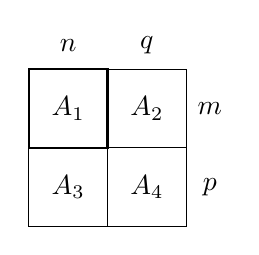
\begin{tikzpicture}[x=1cm, y=1cm]
  \draw (0,1) -- (2,1);
  \draw (1,0) -- (1,2);
  \draw (0,0) -- (2,0) -- (2,2) -- (0,2) -- (0,0);
  \draw[thick] (0,1) rectangle (1,2);
  \draw (0.5,1.5) node{$A_1$};  \draw (0.5,2.3) node{$n$};
  \draw (1.5,1.5) node{$A_2$};  \draw (1.5,2.3) node{$q$};
  \draw (0.5,0.5) node{$A_3$};  \draw (2.3,1.5) node{$m$};
  \draw (1.5,0.5) node{$A_4$};  \draw (2.3,0.5) node{$p$};
\end{tikzpicture}}}}}
\end{align*}
%
%
\vspace{-5.5mm}

\noindent se submaticemi $A_1$ $(m \times n)$, $A_2$ $(m \times q)$,
$A_3$ $(p \times n)$,  $A_4$ $(p \times q)$,
$p \ge 0$, $ q \ge 0$.
%
Sloupce matice $A_1$ nechť jsou lineárně nezávislé. Zpracování
jednotlivých submatic zobecněným ortogonalizačním algoritmem se
vzájemně liší. Budeme proto matici $A$ členit horizontálně
na \Xemph{hlavní a vedlejší submatici} [16] a vertikálně \Xemph{na levou
a pravou submatici}. Vedlejších submatic může být více než jedna,
přičemž mohou mít obecnou polohu vzhledem k hlavní submatici
-- mohou být rozmístěny např. zčásti nad a zčásti pod ní
(kap. 6). Rovněž pravých submatic může být větší počet.
Submatici společnou hlavní a levé submatici budeme označovat jako
\emph{základní.}
%
Ve schematech budeme základní submatici ohraničovat
tučnými čarami.
%
\orig{12}
%
Pokud nebude výslovně uvedeno jinak, budeme ve (2.26) za hlavní
považovat horní submatici $[A_1 ~ A_2]$, za vedlejší pak submatici
$[A_3 ~ A_4]$, příp.\ další submatice umístěné pod ní. Základní submaticí je
potom matice~$A_1$.


Zobecněný ortogonalizační algoritmus spočívá v přetvoření
matice $A$ na matici $W$ o stejné struktuře
%
\begin{align*}
W &= \tag{2.17}{
\vcenter{\hbox{
  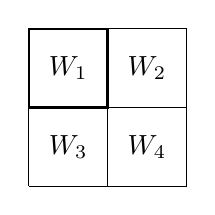
\begin{tikzpicture}[x=1cm,y=1cm]
  \draw (0,1)--(2,1);
  \draw (1,0)--(1,2);
  \draw (0,0) -- (2,0) -- (2,2) -- (0,2) -- (0,0);
  \draw[thick] (0,1) rectangle (1,2);
  \draw (0.5,1.5) node{$W_1$};
  \draw (1.5,1.5) node{$W_2$};
  \draw (0.5,0.5) node{$W_3$};
  \draw (1.5,0.5) node{$W_4$};
\end{tikzpicture}}}}
\end{align*}
%
podle následujících pravidel:
%
\begin{enumerate}
\item {Ortogonalizace levé submatice}.

   Levou submatici matice $A$ transformujeme na levou submatici matice
   $W$ některým z uvedených ortogonalizačních postupů s tím rozdílem, že
   skalární součiny $(a_i,w_j)$ ve ($2.1_2$) resp. $(a_i^{j}.w_j)$ ve
   ($2.1_2$) stejně jako normalizační faktory $\|\widetilde w_i\|$ ve
   ($2.1_3$) počítáme pouze z prvků odpovídajících hlavní submatici.

\item {Ortogonalizace pravé submatice}.

Sloupce pravé submatice matice $A$ převádíme na sloupce pravé
submatice $W$ postupem, který je např. pro metodu GS popsán vzorcem
%
\begin{align*}
%
\tag{2.18}
%
\begin{bmatrix} w_{2_i} \\ w_{4_i} \\ \end{bmatrix}
&=
\begin{bmatrix} a_{2_i} \\ a_{4_i} \\ \end{bmatrix}
-
\sum_{j=1}^n (a_{2_i},w_{i_j})
\begin{bmatrix} w_{1_j}\\ w_{3_j}\end{bmatrix}, \qquad (i=1,2,\ldots,q),
%
\end{align*}
%
kde $a_{s_t}$  ($w_{s_t}$) značí $t$-tý sloupec matice $A_s$ ($W_s$).
Ortogonalizujeme tedy jednotlivé sloupce matice
$
\begin{bmatrix}
   A_2 \\ A_4
\end{bmatrix}
$
ke sloupcům matice
$
\begin{bmatrix}
W_1 \\ W_3
\end{bmatrix},
$
přičemž potřebné skalární součiny počítáme opět pouze z prvků
odpovídajících hlavní submatici a navíc neužíváme normalizace.
Stejné zásady platí i pro metodu MGS.
\end{enumerate}

Při užití zobecněné ortogonalizace se zřejmě zpracování
matice $A_1$ neliší od jejího zpracování běžnou ortogonalizací (2.1)
nebo (2.11). V souladu s (2.10) platí
%
\begin{align*}
   A_1 &= W_1 R.                                            \tag{2.19}
\end{align*}
%
Protože \orig{13} matice $R$ je regulární, odpovídá tedy transformace
$A_1 \rightarrow W_1$
násobení matice $A_1$ maticí $R^{-1}$ zprava. V důsledku toho je
%
\begin{align*}
\tag{2.20}   W_3 = A_3 R^{-1}.
\end{align*}
%
Dále platí
%
\begin{align*}
\tag{2.21}   W_2 &= A_2 - W_1W_1^TA_2 \\
\tag{2.22}   W_4 &= A_4 - W_3W_1^TA_2  = A_4 - A_3R^{-1}W_1^TA_2.\\
\end{align*}
